% !TeX spellcheck = en_US
% !TeX encoding = UTF-8
\documentclass[12pt,aspectratio=43,xcolor={usenames,dvipsnames,table}]{beamer}
\mode<presentation>
\usepackage[T1]{fontenc}
\usepackage[utf8]{inputenc}
\usepackage[english]{babel}
\usepackage{lmodern}
\usepackage[babel,style=english,english=american]{csquotes}
\usepackage{mathabx}
\usepackage{latexsym}
\usepackage{graphicx}
\usepackage{multicol}
\usepackage{multirow}
\usepackage[gen]{eurosym}
\usepackage{pgfpages}
\usepackage{xspace}
\usepackage{appendixnumberbeamer}
\usepackage[binary-units]{siunitx}
\usepackage{tabu}
\usepackage{graphicx}
\usepackage{pgfgantt}
%\usepackage{biblatex}

%\setcounter{tocdepth}{2}

%\usetheme[numbering=counter,progressbar=frametitle]{metropolis}
%\usetheme[numbering=none]{metropolis}
%\usetheme[sectionpage=none,subsectionpage=none,numbering=counter,progressbar=none]{metropolis}
\usetheme[sectionpage=progressbar,subsectionpage=progressbar,numbering=counter,progressbar=frametitle]{metropolis}

\title{Software Development Project}
\subtitle{Final Presentation}
\titlegraphic{
\includegraphics[width=5cm]{gfx/logo}}
\author{Wei-Chan Hsu, Torsten Jandt, Ramesh Kumar, Danning Wang}
\date{July 10, 2017}

\setbeamertemplate{caption}{\raggedright\insertcaption\par}



\setbeamerfont{footnote}{size=\tiny}

\begin{document}

\begin{frame}[noframenumbering,plain]
\titlepage
\end{frame}

% !TeX encoding = UTF-8
% !TeX spellcheck = en_US
% !TeX root = presentation.tex

\section{Introduction}
%\begin{frame}{Software Development Project}
%\begin{itemize}
%	\item Object-oriented software development
%	\item Agile software development
%	\item Unified modeling language (UML) 
%	\item Refactoring
%	\item Software development in robotics
%\end{itemize}

%\end{frame}

\begin{frame}{Basic Navigation Test}
\begin{itemize}
    \item Environment: Workspaces, waypoints and obstacles.
    \item Task specification: Sequence of poses.
\end{itemize}
\centering \includegraphics[height=50mm]{gfx/arena.jpg}
\end{frame}

\begin{frame}{Challenges}
\begin{itemize}
    \item \textbf{Perception:} Accessing and processing sensor data.
    \item \textbf{Mapping:} Building map of the environment.
    \item \textbf{Localization:} Pose inside map.
    \item \textbf{Path planning:} Determine sequence of poses between waypoints.
    \item \textbf{Motion control:} Execution of path.
\end{itemize}
\end{frame}

\begin{frame}{KUKA youBot}
The youBot is a mobile manipulator designed for education and research purposes. It comes with fully open interfaces and API. 
\begin{columns}
    \begin{column}{0.6\textwidth}
        %\begin{block}{System}
        \begin{itemize}
            \item Omnidirectional, four-wheeled
            \item 5-DOF manipulator with a two-finger gripper
            \item On-board PC with CPU, 2GB memory, 32GB SSD drive
            \item Sensors: vision sensors, rangefinders
        \end{itemize} 
        %\centering \includegraphics[width=0.25\textwidth]{slides/gfx/youbot.jpg}   
        %\end{block}
    \end{column}
    \begin{column}{0.4\textwidth} % alternative top-align that's better for graphics
        \centering
        \includegraphics[width=\linewidth]{gfx/youbot.jpg}
    \end{column}
    
\end{columns}
\end{frame}

\begin{frame}[allowframebreaks]{Robot Operating System (ROS)}
Set of software and libraries.
\begin{itemize}
    \item \textbf{Node}: A process using ROS. 
    \item \textbf{Topic}: Message queue, used for communication between nodes.
    \begin{figure}
        \includegraphics[width=0.5\textwidth]{gfx/topic.png}
    \end{figure}
    \item \textbf{Service}: Offers synchronous service calls.
    \begin{figure}
        \includegraphics[width=0.5\textwidth]{gfx/service.png}
    \end{figure}
    \item \textbf{Actionlib} 
    \begin{itemize}
        \item Provides client interface to send requests to server
        \item Client and server communicate with messages:
        \begin{itemize}
            \item Goal
            \item Feedback
            \item Result
        \end{itemize}
    \end{itemize} 
\end{itemize}
\end{frame}

% !TeX encoding = UTF-8
% !TeX spellcheck = en_US
% !TeX root = presentation.tex

\section{Approach}
\begin{frame}{Software Modules}
    \begin{center}
        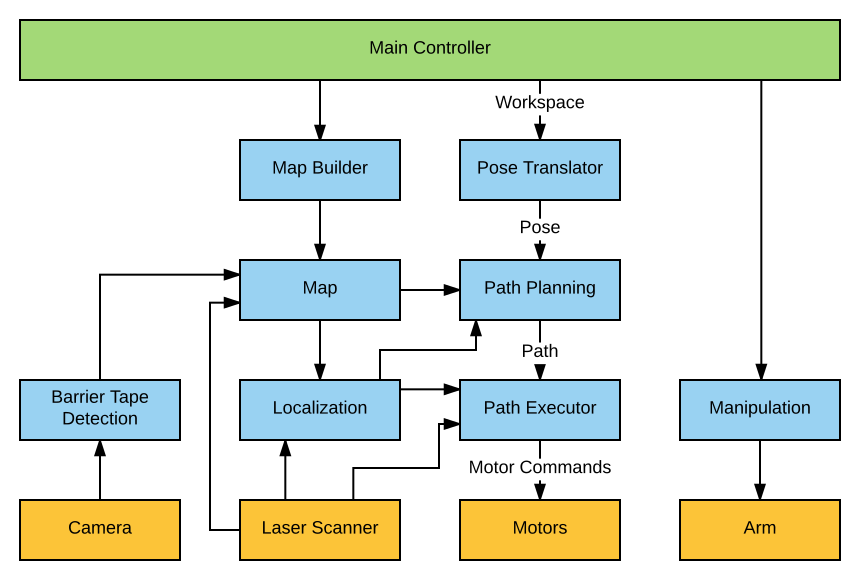
\includegraphics[width=\linewidth,height=0.9\textheight,keepaspectratio]{gfx/software_modules.pdf}
    \end{center}
\end{frame}

\section{Realization}
% !TeX encoding = UTF-8
% !TeX spellcheck = en_US
% !TeX root = presentation.tex

\subsection{Simulation}

\begin{frame}{Simulation}
    \begin{itemize}
        \item Simple Two Dimensional Robot (STDR) simulator	
        \item Tasks  performed:
        \begin{itemize}
            \item Map Building
            \item Localization
        \end{itemize}
    \end{itemize}
    
    \centering
    \includegraphics[width=90mm,height=55mm]{gfx/stdr_simulator}
    
\end{frame}
%---------------------------------------------------------------
\begin{frame}{Map building I}
    \begin{itemize}
        \item Gmapping is used to build 2D occupancy grid map 
		\item Uses laser sensors to build the map
        \item Map Server
        \begin{itemize}
            \item Provides map saver utility, to save generated map in files(yaml and pgm)
            \item Offers map data as a ROS Service
        \end{itemize}
        
    \end{itemize}
\end{frame}
%-----------------------
\begin{frame}{Map building II}
    \begin{center}
    \includegraphics[width=0.6\textwidth]{gfx/frames_cleaned.pdf}
    \end{center}
\end{frame}
%----------------------------------------------------------------
\begin{frame}{Localization I}
    \begin{itemize}
        \item Adaptive Monto Carlo Localization(AMCL) is used to localize the robot
        \item Uses particle filter to track the pose of robot

        \item Problems:
        \begin{itemize}
            \item AMCL could not find laser data on /scan topic
            \item AMCL node crushes after some time
            
        \end{itemize}
        \item Solutions:
        \begin{itemize}
            \item Remap /scan\_front and /scan\_rear to /scan topic
            \item Because of transformations provided by STDR simulator
            
        \end{itemize}
    \end{itemize}
\end{frame}
% !TeX encoding = UTF-8
% !TeX spellcheck = en_US
% !TeX root = presentation.tex
\subsection{KUKA youBot}
\begin{frame}{youBot Driver}

\begin{itemize}
	\item \textbf{ROS Wrapper}
	\begin{itemize}
		\item Allows to write ROS programs for controlling youBot
		\item Provides an interface between youBot driver and ROS framework
		\item Allows to move the base and arm by sending ROS messages
	\end{itemize}
	\item \textbf{List of Drivers}
		\begin{itemize}
			\item Drive base
			\item Laser scanners
			\item Arm 
			\item Joystick
			\item Transformations
		\end{itemize}
\end{itemize}
  
\end{frame}

%-----------------------
\begin{frame}{Map building II}
\begin{itemize}
	\item \textbf{Problems}
		\begin{itemize}
			\item Messy Map
		\end{itemize}
	\item \textbf{Solutions}
		\begin{itemize}
			\item Incorrect transformation between laser frame and base link
		\end{itemize}
\end{itemize}
\end{frame}
%-----------------------
\begin{frame}{Map building III}
    \centering
    \includegraphics[width=0.9\textwidth]{gfx/map_messy.png}
\end{frame}
\begin{frame}{Map building IV}
\centering
\includegraphics[width=0.8\textwidth]{gfx/map.png}
\end{frame}
%-----------------------
\begin{frame}{Localization II}
\end{frame}
%-----------------------
\begin{frame}{Navigation}
\begin{itemize}
	\item Requirements
		\begin{itemize}
			\item Map (map\_server)
			\item Localization (amcl)
			\item Odometry source
			\item Transforms
			\item Sensor sources
			\item Goal (move\_base) 
		\end{itemize}
	\item Components
		\begin{itemize}
			\item Planners: global, local
			\item Costmaps: global, local
		\end{itemize}
	\item Output: Velocity command (cmd\_vel)
\end{itemize}
\end{frame}
%-----------------------
\begin{frame}{Navigation - Local Planner}
\begin{itemize}
	\item Planner: dwa\_local\_planner
	\item Given: plan, costmap, odom
	\item Generates costs of transversing through map grids
	\item Output: Velocity command
\end{itemize}
\end{frame}
%-----------------------
\begin{frame}{BNT.py}
    
    The node acts as path executor that reads  a set of user inputs and convert them to move\_base\_msgs.
    \begin{itemize}
        \item Class: Position, Pose, Environment, Workspace, PathExecutor
        
        \item Functions:
        \begin{itemize}
        	\item Reads user inputs
        	\item Reads workspace from file
            \item Converts workspace to move\_base\_msgs
            \item Clears cost map
            \item Sends goal message
        \end{itemize}
    \end{itemize}
    
\end{frame}

% !TeX encoding = UTF-8
% !TeX spellcheck = en_US
% !TeX root = presentation.tex

\section{Results}
\begin{frame}{Launch Files}
    \centering
    \includegraphics[width=\textwidth]{gfx/launchfile.png}
\end{frame}
\begin{frame}{RQT Graph}
    \centering
    \includegraphics[width=\textwidth]{gfx/rosgraph}
\end{frame}

\begin{frame}{Class Diagram}
    \begin{center}
        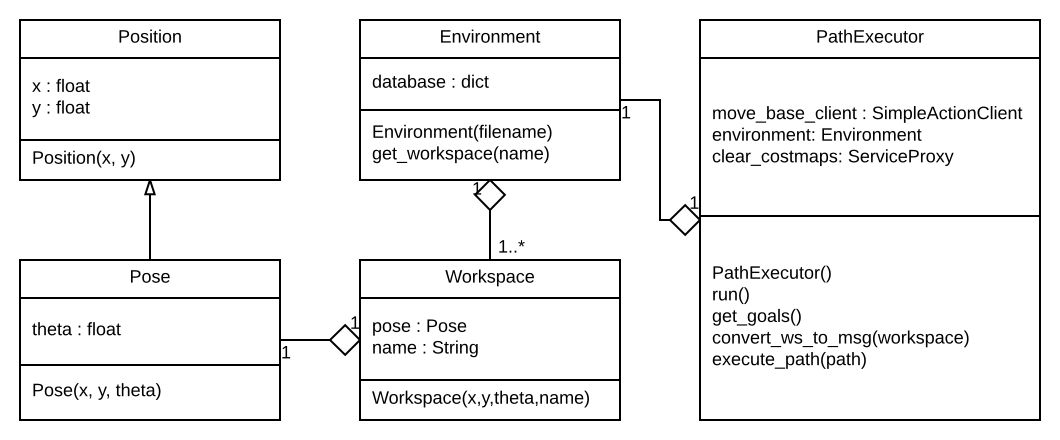
\includegraphics[width=\linewidth,height=0.9\textheight,keepaspectratio]{gfx/01.pdf}
    \end{center}
\end{frame}


\begin{frame}{Sequence Diagram}
    \begin{center}
        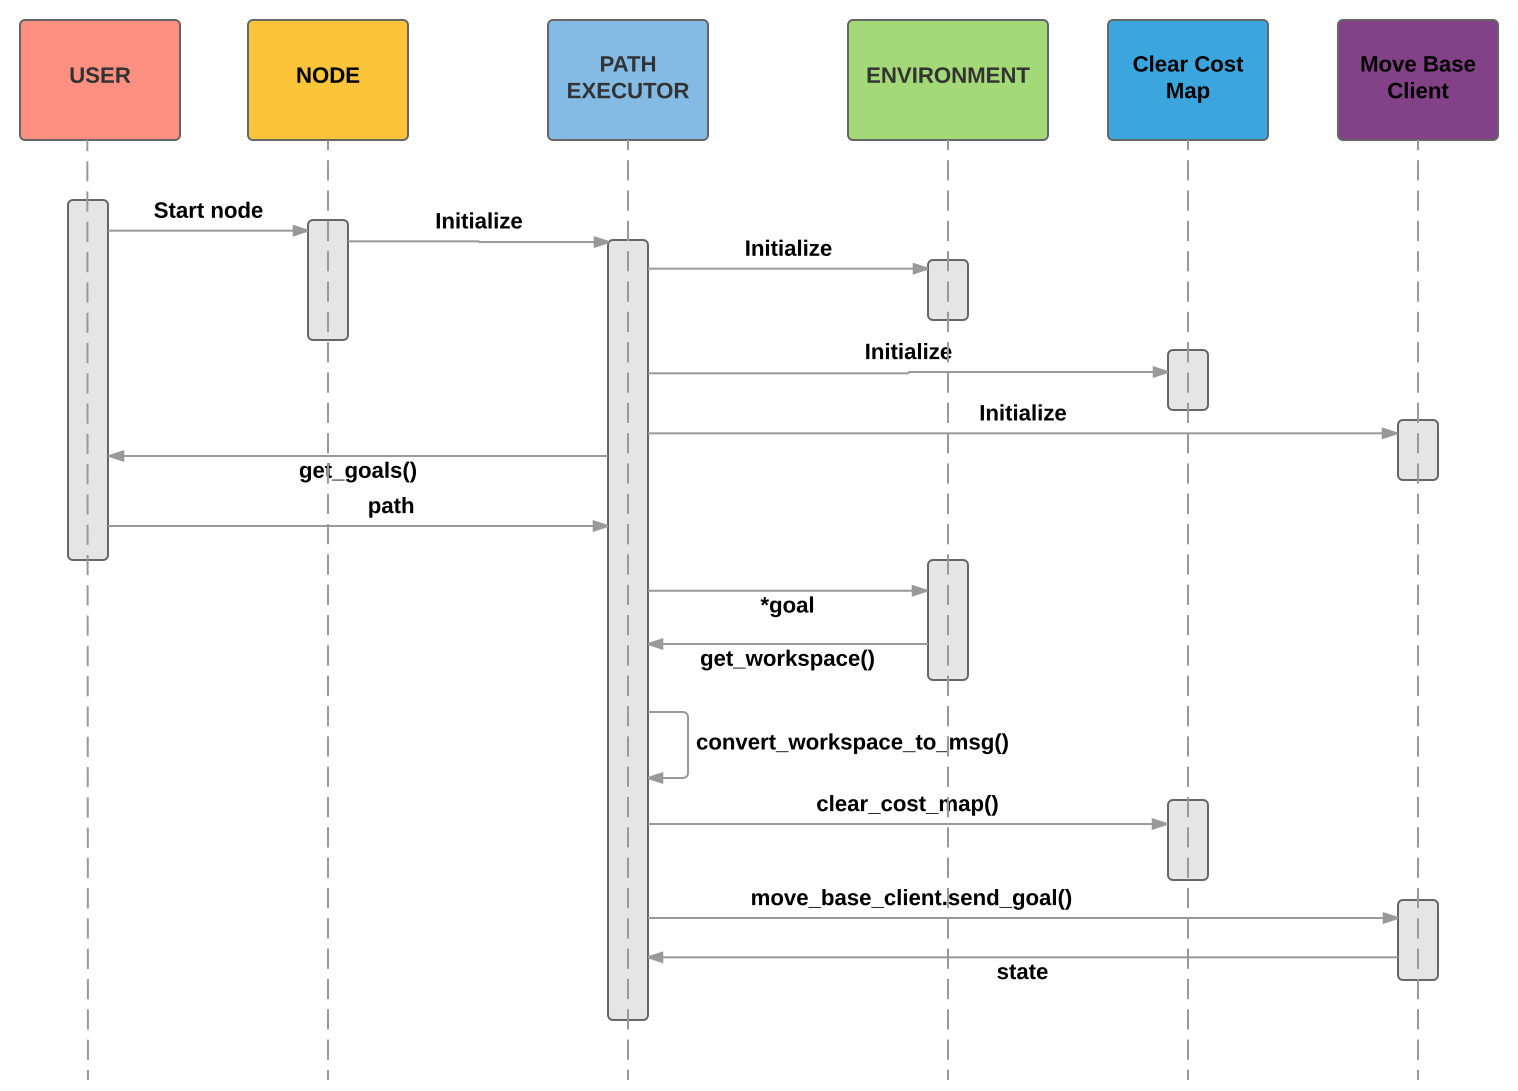
\includegraphics[width=\linewidth,height=0.9\textheight,keepaspectratio]{gfx/02.pdf}
    \end{center}
\end{frame}
% !TeX encoding = UTF-8
% !TeX spellcheck = en_US
% !TeX root = presentation.tex

\section{Conclusions}
\begin{frame}{Conclusions}
\begin{itemize}
	\item Navigation was analyzed and applied to youBot.    
	\item The task contains mapping, localization, path planning, motion execution.
	%\item Mapping was realized using gmapping, which requires laser scans and correct transforms.
	%\item Localization was achieved using AMCL, which relies on a map, laser scans, transforms, and initial pose.
	%\item DWA local planner was employed for path-planning.
	\item A node was created as a path executor that requests user input. 
	\item The robot was able to navigate around the lab by user input of a series of workspace.
    \item We faced some problems, most of them are solved.
\end{itemize}
\end{frame}
\begin{frame}{Future Work}
\begin{itemize}
	\item User interface can be improved.
	\item The parameters can be tuned to improve the performance of robot.
    \item Barrier tape detection
    \begin{itemize}
        \item Arm control
        \item Process camera data
    \end{itemize}
\end{itemize}
\end{frame}

\end{document}